\RequirePackage{fix-cm}
\documentclass[10pt,letterpaper]{article}

\usepackage[margin=0.52in]{geometry}
\usepackage{graphicx}
\usepackage{amsmath}
\usepackage{caption}
\usepackage{times}

\graphicspath{{../}}
\setlength{\parindent}{0pt}
\setlength{\parskip}{3pt}
\captionsetup{font=scriptsize,labelfont=bf,skip=2pt}

\begin{document}
\fontsize{9.2}{10.6}\selectfont

\begin{center}
{\Large\bfseries Device-Guided Stanford RRAM Model Extraction for\\[-1pt]
Sputter-Deposited TaO$_x$ Devices}\\[3pt]
Md Tawsif Rahman Chowdhury, Alireza Moazzeni, and Gozde Tutuncuoglu\\
Department of Electrical and Computer Engineering, Wayne State University
\end{center}

\section*{Summary and Motivation}
We calibrated the Stanford--PKU RRAM compact model to measured DC switching
data from sputter-deposited TaO$_x$ devices fabricated under twelve oxygen
flow and RF sputter-power conditions.  The goal was not only to obtain a good
simulated $I$--$V$ overlay.  For a semiconductor modeling and fabrication
group, the more important question is: \emph{which fitted parameters can be
trusted as deposition-dependent information, and which are only numerical
knobs that help the curve fit?}

This distinction matters because the Stanford model has many adjustable
parameters, while a DC butterfly sweep contains only a limited number of
visible features: the low- and high-resistance branches, SET and RESET
transition voltages, branch curvature, and current compliance region.  Many
parameter combinations can reproduce these features.  Therefore, a good
overlay is necessary for circuit use, but it does not automatically prove that
each extracted parameter has physical meaning.

Our extraction flow adds two simple checks after fitting.  First, we test
whether a model fitted to one representative cycle predicts all other measured
cycles of the same device.  This tells us whether the fit represents the
device population rather than only one selected trace.  Second, we repeatedly
resample the measured cycles and refit the model.  This is called a
bootstrap; here it simply means ``refit many slightly different cycle
populations and see which parameters stay stable.''  A stable parameter is
useful for interpretation.  A parameter that moves widely is treated as a
fitting degree of freedom, not a process metric.

\section*{Device Set and Methodology}
The devices are sputter-deposited TaO$_x$ cross-point RRAM cells with
\(4~\mu\mathrm{m}\) feature size.  Twelve sample conditions span oxygen
percentage in the sputter ambient and RF sputter power, including four
replicated center-point conditions.  This design allows deposition trends to
be checked, but only for parameters that are repeatably extracted.

The extraction flow has four main steps.  First, measured cycles are screened
to reject shorted, open, incomplete, or noise-floor sweeps.  Second, one
representative measured cycle is selected automatically.  We use the
\emph{medoid}, which is the real measured cycle closest to the median
cycle behavior.  This avoids hand-picking a visually attractive curve and also
avoids fitting an artificial averaged loop.

Third, before compact-model fitting, each resistance-state segment is
classified as ohmic, Poole--Frenkel, Schottky, or Fowler--Nordheim.  This is a
device-physics front end.  Ohmic and Poole--Frenkel-like regions are closest
to what the released Stanford current law can represent.  Schottky and
Fowler--Nordheim regions are still reported and validated, but they are
treated as possible model-mismatch regions during fitting.  This prevents
interface-limited HRS behavior from forcing unrelated bulk-model parameters
to compensate.

Fourth, the Stanford Verilog-A model is fitted using HSPICE simulations.  The
objective compares measured and simulated currents on a log-current scale,
because the current spans many decades.  The search is guided by physically
reasonable parameter ranges and by the conduction classification.  In plain
language, the algorithm searches broadly enough to fit the data, but it is
discouraged from using unsupported parameters to hide missing physics.

\newpage

\section*{Results and Interpretation}
The first result is a device-physics result.  The post-SET low-resistance
state is consistently ohmic, as expected for a conductive filament branch.
The post-RESET high-resistance state (HRS) is Schottky-dominant in
92.5--100\% of cycles for all twelve conditions.  The extracted dynamic
permittivity values are physically admissible, supporting the conclusion that
the HRS is interface-limited rather than simply noisy or poorly fitted.  This
also explains why RESET remains harder to fit: the released Stanford model
does not explicitly include a Schottky barrier current.

The fitted models reproduce the measured DC switching loops with mean
log-current RMSE of 0.530 decades for SET and 0.761 decades for RESET.  The
dominant residuals occur near the switching transition and along the
Schottky-limited HRS approach.  Thus, the remaining error is mainly a
model-adequacy issue, not a failure of the optimizer.

The out-of-sample cycle test shows that the model generalizes.  When the
parameter set fitted to one medoid cycle is scored against every other
measured cycle of the same device, the held-out median errors are 0.542
decades for SET and 0.800 decades for RESET.  These are very close to the
fitted-cycle errors.  Therefore, the extracted model is a behavioral
description of the device cycle population, not just a memorized overlay of
one trace.

The bootstrap analysis shows which parameters can be interpreted.  The branch
voltage scales are the most repeatable quantities and carry meaningful
deposition trends.  This is reasonable because these voltage scales directly
control branch curvature in the measured $I$--$V$ curve.  In contrast, series
resistance and velocity prefactors vary strongly when the measured cycles are
resampled.  They may be needed to produce a good fit, but they should not be
reported as standalone deposition-dependent physical parameters from these DC
sweeps.

\section*{Novel Contributions}
The work makes four contributions.  First, it reframes Stanford-model
calibration as a device-facing extraction problem: the deliverable is not only
a curve overlay, but also evidence that the fit generalizes and that selected
parameters are repeatable.  Second, it places conduction-regime classification
before fitting, so the method knows where the TaO$_x$ data follow the compact
model and where interface-limited HRS transport lies outside it.  Third, it
shows that a single medoid-cycle calibration predicts the full measured cycle
population of the same device.  Fourth, it separates deposition-useful
parameters from fit-only parameters: branch voltage scales are usable for
process comparison, while series resistance, velocity prefactors, activation
energies, and several gap-related quantities are not repeatable enough for
physical interpretation from DC data alone.

\section*{Conclusion}
For these sputter-deposited TaO$_x$ RRAM devices, a good compact-model overlay
is only the first checkpoint.  The fitted Stanford model is useful as a
behavioral model because it predicts held-out measured cycles with nearly the
same error as the fitted cycle.  However, the extracted parameter table must
be interpreted selectively.  Only repeatable quantities, especially the branch
voltage scales, should be used to discuss deposition dependence.  The
post-RESET HRS is consistently Schottky-limited, which sets the RESET error
floor and points to a clear model-extension direction: adding an
interface-limited HRS current branch.  The central message is that RRAM model
extraction for fabrication studies should report fit quality, missing device
physics, cycle-level generalization, and parameter repeatability together.

\clearpage

\section*{Figures}
\vspace{-5pt}
\begin{center}
\begin{minipage}{0.49\textwidth}
\centering
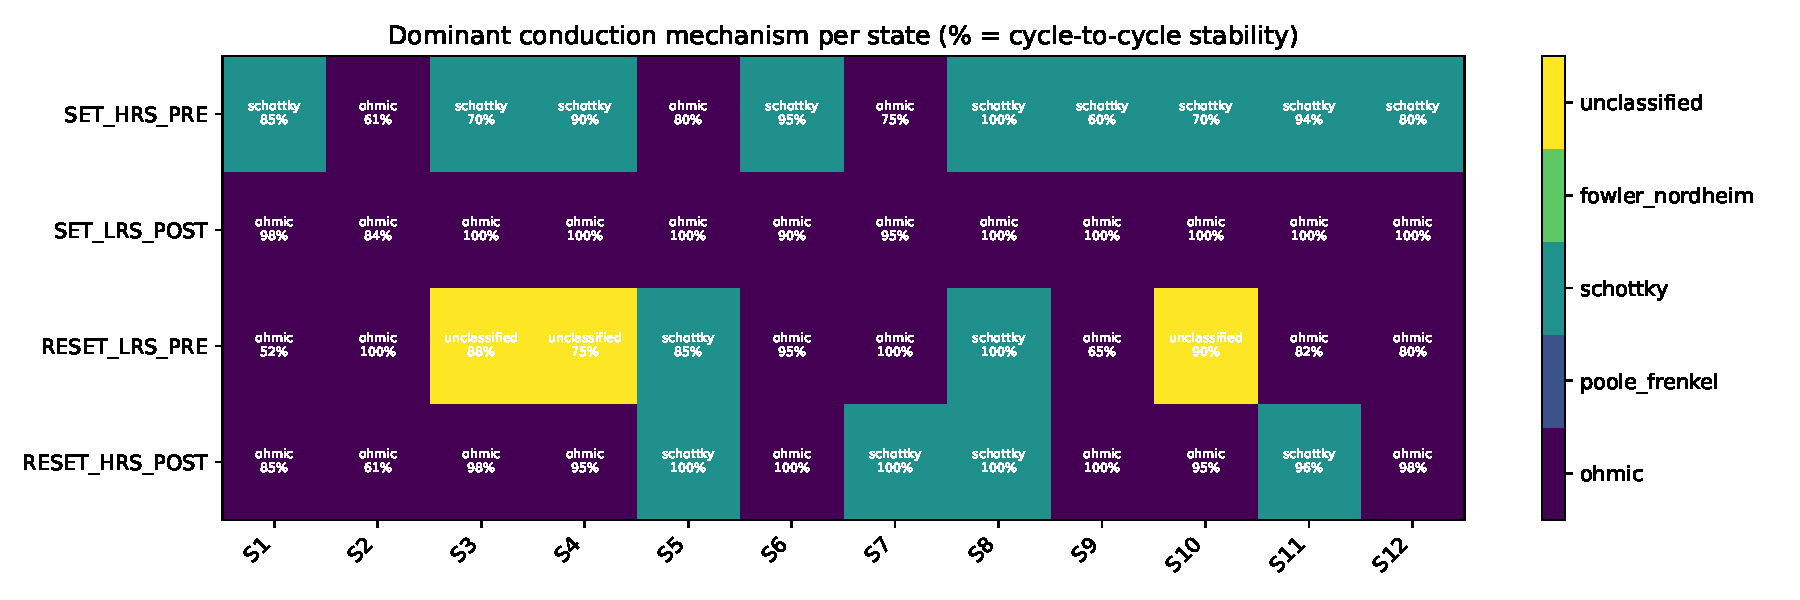
\includegraphics[width=\linewidth,height=0.265\textheight,keepaspectratio]{results/variability/mechanism_map.pdf}
\captionof{figure}{Dominant conduction mechanism for each state segment and
deposition condition.  The main pattern is the device story: post-SET LRS is
mostly ohmic, while post-RESET HRS is Schottky-like for essentially all
conditions.  This identifies the HRS region where the Stanford current law is
missing interface-barrier physics.}
\end{minipage}\hfill
\begin{minipage}{0.49\textwidth}
\centering
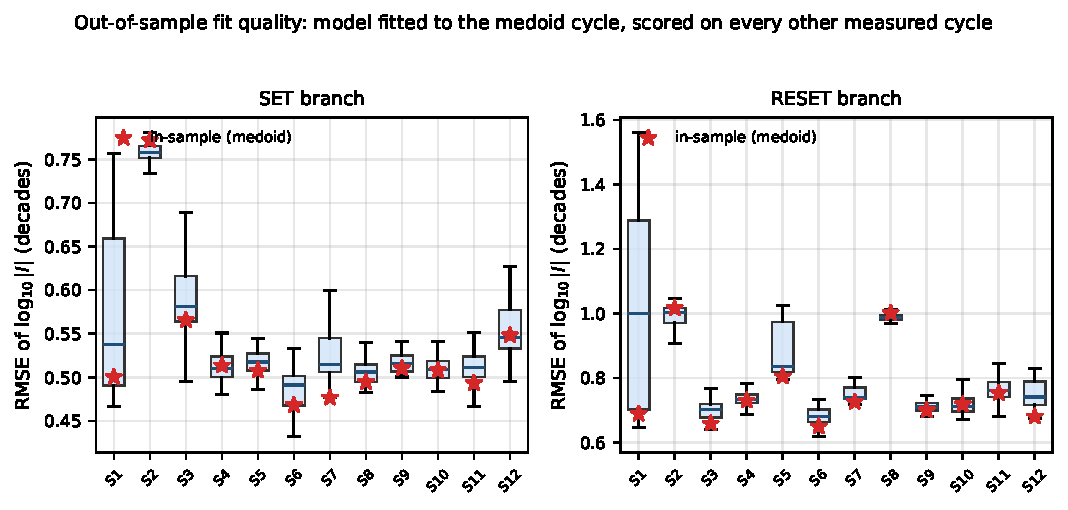
\includegraphics[width=\linewidth,height=0.265\textheight,keepaspectratio]{results/paper_alt/heldout_rmse.pdf}
\captionof{figure}{Out-of-sample cycle test.  Boxes show the error when the
medoid-cycle fit is evaluated on other measured cycles; stars show the fitted
cycle.  The overlap means the parameter set describes the measured cycle
population rather than only the selected fitting trace.}
\end{minipage}

\vspace{8pt}
\begin{minipage}{0.49\textwidth}
\centering
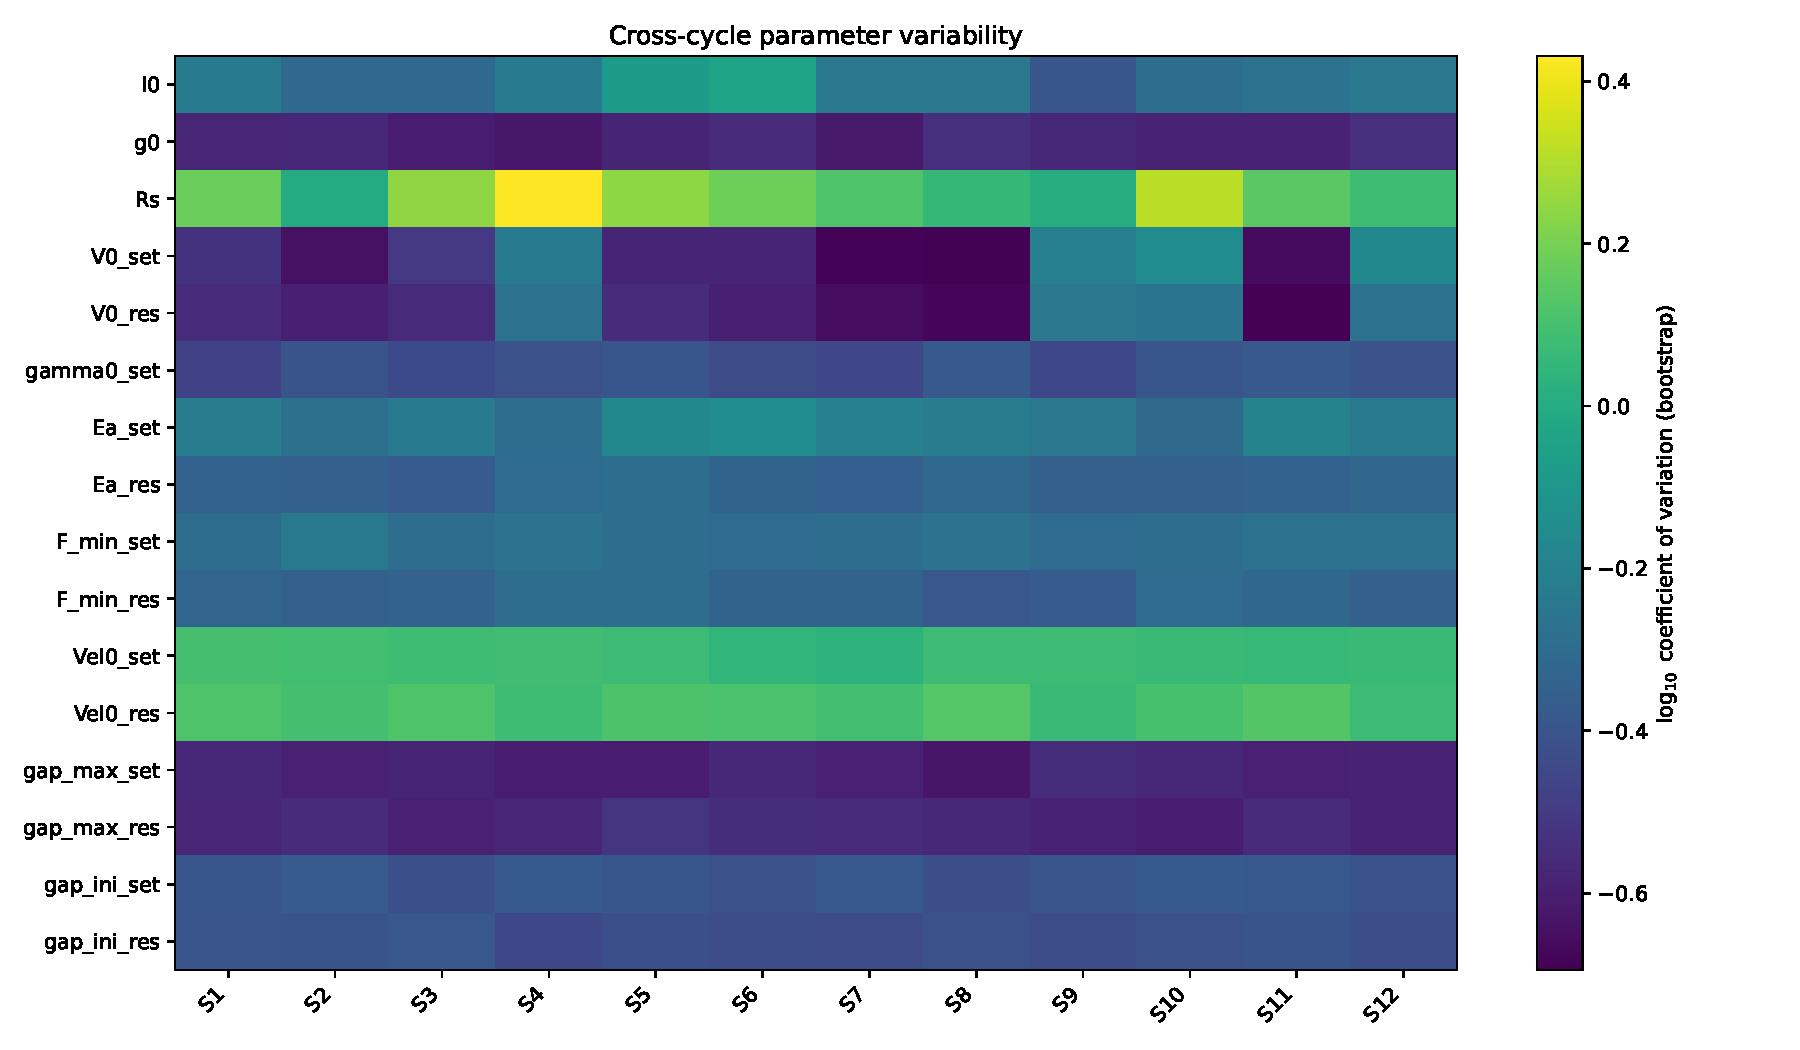
\includegraphics[width=\linewidth,height=0.265\textheight,keepaspectratio]{results/variability/parameter_cv.pdf}
\captionof{figure}{Bootstrap parameter variability.  Low CV means repeatable
extraction.  Branch voltage scales are stable, while series resistance and
velocity prefactors vary strongly under cycle resampling and should be treated
as fit-only quantities for these DC sweeps.}
\end{minipage}\hfill
\begin{minipage}{0.49\textwidth}
\centering
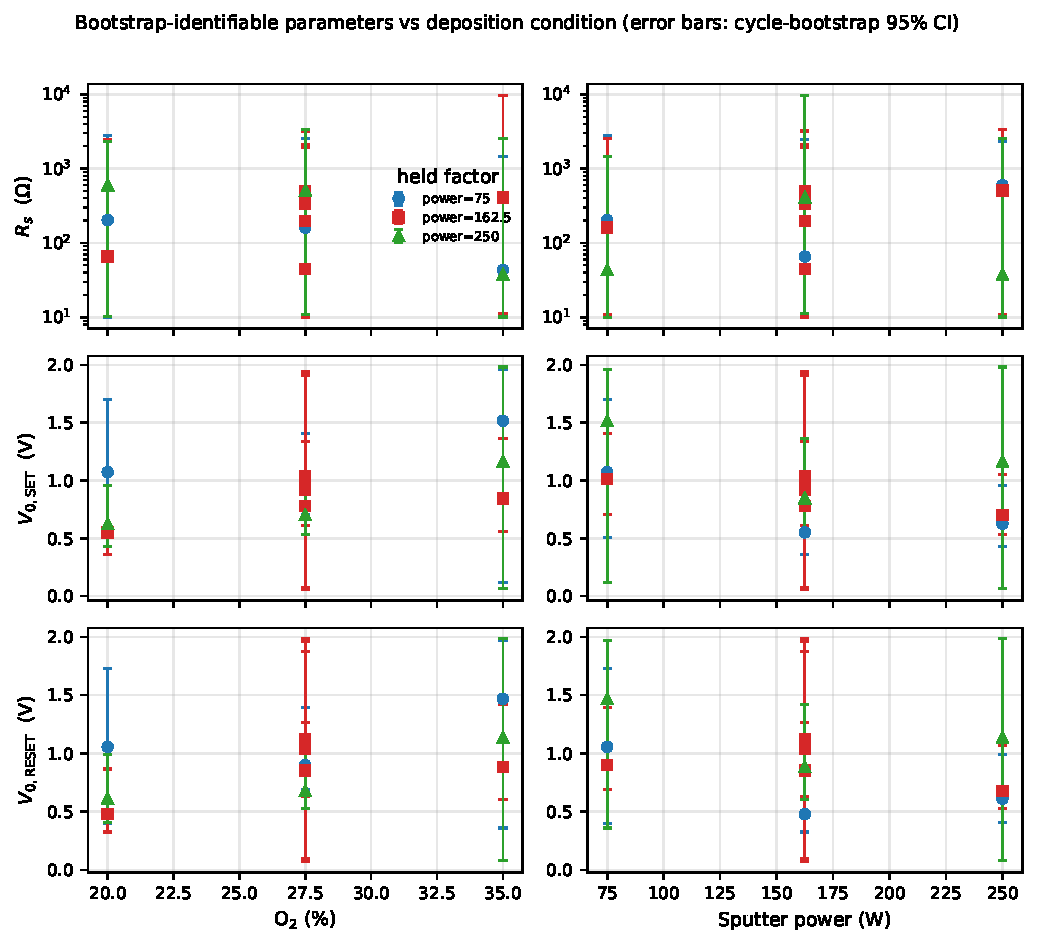
\includegraphics[width=\linewidth,height=0.265\textheight,keepaspectratio]{results/paper_alt/deposition_trends.pdf}
\captionof{figure}{Deposition-resolved extraction.  Branch voltage scales have
tighter bootstrap intervals and carry useful deposition information.  Series
resistance spans orders of magnitude, so its apparent process trend is not
reliable from this data set.}
\end{minipage}
\end{center}

\end{document}
